\documentclass[./blockchain.tex
\usepackage{stmaryrd}
\graphicspath{{\subfix{./figures/}}}


\begin{document}

    \section{Kryptographie und weitere Eigenschaften}

    \begin{frame}{Hash-Funktionen}{Was ist eine Hash-Funktion?}
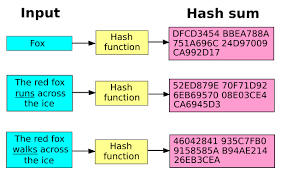
\includegraphics[height=0.3\textheight]{hashfunction}
        \begin{itemize}
            \item 'Fingerabdruck' eines Datenpakets
            \item Hash-Funktion: $Datenpaket \rightarrow 256BinArray$ (Hash-Wert)
            \item Die Hash-Funktion ist nicht eindeutig!
            \item Für eine gute Hash-Funktion ist es jedoch fast unmöglich ein Datenpaket für einen vorgegebenen Hash-Wert zu finden!
        \end{itemize}



    \end{frame}


    \begin{frame}
        \frametitle{Coins, Buchhaltung, Transaktionen}

        \begin{itemize}
            \item Fast alle Blockchains führen einen Coin (Wert, Token).
            \item Die Coins sind buchhalterisch Konten zugewiesen.
            \item Die Anzahl Coins kann je nach Blockchain steigen (mint), sinken (burn) oder gleich bleiben.
            \item Die Blockchain bietet einen built-in Transaktionsmechanismus an.
            \item Die Blockchain stellt sicher, dass es zu keiner willkürlichen 'Vermehrung' kommt.
        \end{itemize}
    \end{frame}


    \begin{frame}
        \frametitle{Wallet, öffentlicher, privater Schlüssel}

        \begin{itemize}
            \item Wallet besteht aus privatem und öffentlichem Schlüssel
            \item Verlust des privaten Schlüssel $\rightarrow$ Verlust des Vermögens
            \item Transaktion: Signierte Überweisung $\rightarrow$ Blockchain
            \item Eine Überweisung kann nicht verweigert werden
        \end{itemize}
    \end{frame}


\end{document}

